\documentclass[twoside,10pt]{article}
\usepackage{amsmath,amsfonts,amsthm,fullpage,amssymb}
%\usepackage{mymath}
\usepackage{algorithm}
\usepackage{algorithmic}
\usepackage{graphicx}
\usepackage{url}


\begin{document}


\title{ISYE 6740 Homework 7 (Last Homework)\\ 
\small Total 100 points.}
%\author{Yao Xie}
%\date{Deadline: Feb. 13, Sat., 11:55pm}
\date{}
\maketitle



As usual, please submit a report with sufficient explanation of your answers to each the questions, together with your code, in a zip folder.

%----------------------------------------------------------------------------------

%\begin{enumerate}

\section{Random forrest for email spam classifier (30 points)}

Your task for this question is to build a spam classifier using the UCR email spma dataset \url{https://archive.ics.uci.edu/ml/datasets/Spambase} came from the postmaster and individuals who had filed spam. The collection of non-spam e-mails came from filed work and personal e-mails, and hence the word \textsf{'george'} and the area code \textsf{'650'} are indicators of non-spam. These are useful when constructing a personalized spam filter. 

One would either have to blind such non-spam indicators or get a very wide collection of non-spam to generate a general purpose spam filter. Load the data. %You will see there are total of 4601 instances, and 57 features. 

\begin{enumerate}

\item (5 points) How many instances of spam versus regular emails are there in the data? How many data points there are? How many features there are?

Note: there may be some missing values, you can just fill in zero.

\item (10 points) Build a classification tree model (also known as the CART model). In Python, this can be done using \textsf{sklearn.tree.DecisionTreeClassifier}. In our answer, you should report the tree models fitted similar to what is shown in the ``Random forest'' lecture, Page 16, the tree plot. In Python, getting this plot can be done using \textsf{sklearn.tree.plot\_tree} function. 

\item (15 points)
Also build a random forrest model. In Python, this can be done using\\ \textsf{sklearn.ensemble.RandomForestClassifier}. 

Now partition the data to use the first 80\% for training and the remaining 20\% for testing. Your task is to compare and report the AUC  for your classification tree and random forest models on testing data, respectively. To report your results, please try different tree sizes. Plot the curve of AUC versus Tree Size, similar to Page 15 of the Lecture Slides on ``Random Forest''. 


{\it Background information:} In classification problem, we use AUC (Area Under The Curve) as a performance measure. It is one of the most important evaluation metrics for checking any classification model?s performance. ROC (Receiver Operating Characteristics) curve measures classification accuracy at various thresholds settings. AUC measures the total area under the ROC curve. Higher the AUC, better the model is at distinguishing the two classes. If you want to read a bit more about AUC curve, check out this link \url{https://towardsdatascience.com/understanding-auc-roc-curve-68b2303cc9c5} For instance, in Python, this can be done using \textsf{sklearn.metrics.roc\_auc\_score} and you will have to figure out the details. 

\end{enumerate}


\section{Nonlinear regression and cross-validation (30 points)}


The coefficient of thermal expansion $y$ changes with temperature $x$. An experiment to relate $y$ to $x$ was done. Temperature was measured in degrees Kelvin. (The Kelvin temperature is the Celcius temperature plus 273.15). The raw data file is \textsf{copper-new.txt}.

\begin{figure}[h!]
\begin{center}
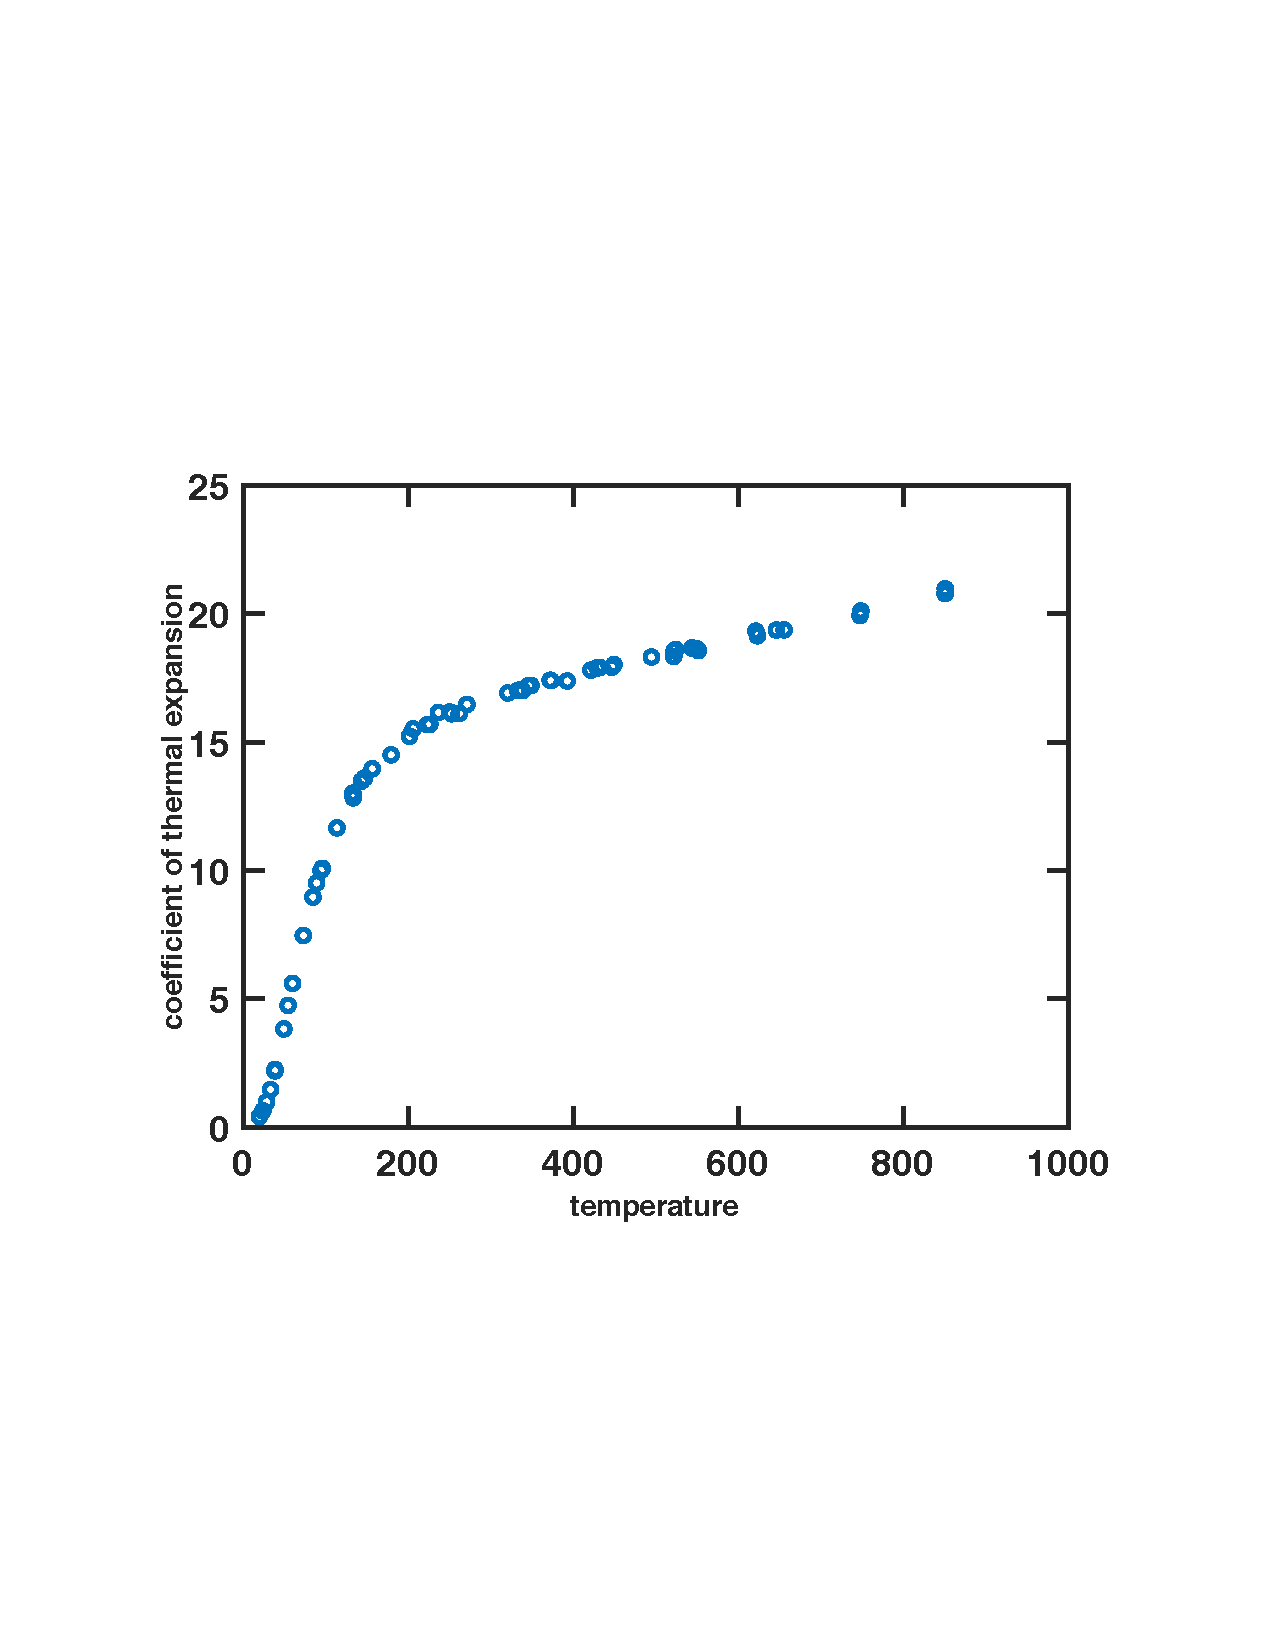
\includegraphics[width = 0.6\textwidth]{t_c}
\end{center}
\end{figure}

\begin{enumerate}

\item (10 points) Perform linear regression on the data. Report the fitted model and the fitting error.
\item (10 points) Perform nonlinear regression with polynomial regression function up to degree $n = 10$ and use ridge regression (see Lecture Slides for ``Bias-Variance Tradeoff''). Write down your formulation and strategy for doing this, the form of the ridge regression. 
\item (5 points) Use $5$ fold cross validation to select the optimal regularization parameter $\lambda$. Plot the cross validation curve and report the optimal $\lambda$.
\item (5 points) Predict the coefficient at 400 degree Kelvin using both models. Comment on how would you compare the accuracy of predictions. 
%\item What is an upper bound for the prediction error at this 400 degree point? 
\end{enumerate}



\section{Regression, bias-variance tradeoff (40 points)} 

%(Bonus question. 10 points.) 

Consider a dataset with $n$ data points $(x_i, y_i)$, $x_i \in \mathbb R^p$, drawn from the following linear model:
\[
y = x^T {\beta^*} + \epsilon,
\]
where $\epsilon$ is a Gaussian noise and the star sign is used to differentiate the true parameter from the estimators that will be introduced later. Consider the regularized linear regression as follows:
\[
\hat \beta(\lambda) 
= \arg\min_{\beta}
\left\{
\frac 1 n \sum_{i=1}^n (y_i -x_i^T \beta)^2 + \lambda \|\beta\|_2^2
\right\},
\]
where $\lambda \geq 0$ is the regularized parameter. Let $X\in \mathbb R^{n\times p}$ denote the matrix obtained by stacking $x_i^T$ in each row. 
\begin{enumerate}
\item (10 points) Find the closed form solution for $\hat \beta(\lambda)$ and its distribution.
\item (10 points) Calculate the bias  $\mathbb E[x^T {\hat \beta}(\lambda)] - x^T {\beta^*}$ as a function of $\lambda$ and some fixed test point $x$.
\item (10 points) Calculate the variance term $\mathbb E\left[\left(x^T {\hat \beta}(\lambda) - \mathbb E[x^T {\hat \beta}(\lambda)] \right)^2\right]$.
\item (10 points) Use the results from parts (b) and (c) and the bias-variance decomposition to analyze the impact of $\lambda$ in the squared error. Specifically, which term dominates when $\lambda$ is small, and large, respectively?
\end{enumerate}


(Hint.) Properties of an affine transformation of a Gaussian random variable will be useful throughout this problem.


\end{document}
